\documentclass[journal]{IEEEtran}
\usepackage{graphicx}
\usepackage[outdir=./]{epstopdf}
%\usepackage{subfigure}

\usepackage{subcaption}
\usepackage{hyperref}
\usepackage{booktabs}
\usepackage[table]{xcolor}
\usepackage{multirow}
\usepackage{cleveref}
\usepackage[utf8]{inputenc}
\usepackage[spanish, mexico]{babel}

\usepackage{amsmath}
\usepackage{algorithm}
\usepackage{algorithmic}
\input{spanishAlgorithmic}

\usepackage{color}
\usepackage{listings}
\lstset{ %
language=Matlab,                % choose the language of the code
basicstyle=\footnotesize,       % the size of the fonts that are used for the code
numbers=left,                   % where to put the line-numbers
numberstyle=\footnotesize,      % the size of the fonts that are used for the line-numbers
stepnumber=1,                   % the step between two line-numbers. If it is 1 each line will be numbered
numbersep=5pt,                  % how far the line-numbers are from the code
backgroundcolor=\color{white},  % choose the background color. You must add \usepackage{color}
showspaces=false,               % show spaces adding particular underscores
showstringspaces=false,         % underline spaces within strings
showtabs=false,                 % show tabs within strings adding particular underscores
frame=single,           % adds a frame around the code
tabsize=2,          % sets default tabsize to 2 spaces
captionpos=b,           % sets the caption-position to bottom
breaklines=true,        % sets automatic line breaking
breakatwhitespace=false,    % sets if automatic breaks should only happen at whitespace
escapeinside={\%*}{*)}          % if you want to add a comment within your code
}

%\usepackage{float}
\usepackage{fourier}
\begin{document}

% Corregir problemas de separación de palabras por guiones
%\hyphenation{op-tical net-works semi-conduc-tor}

\floatname{algorithm}{Pseudocódigo}
\title{Red Neuronal de base radial (\emph{RBFN})}

\author{Rafael~Pérez~Torres \\
	Profesor: Dr. Wilfrido Gómez Flores,\\[6pt]\IEEEmembership{LTI Cinvestav}.
	
	%\thanks{Rafael Pérez Torres es estudiante de doctorado en Ciencias de la Computación en el Laboratorio de Tecnologías de Información del CINVESTAV, email: rperez@tamps.cinvestav.mx.}
}

\markboth{Reconocimiento de patrones, Abril~2015}%
{Pérez Torres: Reconocimiento de patrones}

\maketitle

\begin{abstract}
Las redes neuronales de función de base radial (RBFN) son una alternativa  al perceptrón multicapa.
A diferencia del perceptrón multicapa, las redes neuronales de función de base radial no requieren realizar la retro-propagación del error para realizar el ajuste de los pesos y además mantienen una estructura fija compuesta de una capa de entrada, una capa escondida y una de salida.

Este tipo de redes resultan útiles para aproximar funciones y además realizar la clasificación de patrones.

En este documento se presenta la implementación del entrenamiento híbrido y clasificación utilizando una red neuronal de función de base radial.
El entrenamiento se ha realizado variando la cantidad de neuronas en la capa oculta, así como la función de media utilizada para realizar el cálculo de los radios.
Se muestran las regiones particionadas generadas por las mejores configuraciones obtenidas durante el entrenamiento.
\end{abstract}

\begin{IEEEkeywords}
Reconocimiento de patrones, Redes neuronales de función de base radial, RBFN
\end{IEEEkeywords}

\section{Introducción}
\label{sec:introduccion}

Las redes funcionales de función de base radial surgen como un método alternativo al perceptrón multicapa, siendo propuestas por Broomhead y Lowe en el año de 1988.

Este tipo de redes definen una topología fija consistente en las siguientes capas:
\begin{itemize}
	\item \textbf{Entrada}: recibe y distribuye los datos desde el exterior.
	\item \textbf{Oculta}: activada por funciones radiales \emph{no lineales}.
	\item \textbf{Salida}: activada por funciones \emph{lineales} continuas.
\end{itemize}

La salida de este tipo de redes está definida por una transformación no lineal en la capa oculta y una lineal en la capa de salida.
Existen múltiples funciones de transformación no lineal.
Dentro de las más comunes se encuentran
\begin{itemize}
	\item Función Gaussiana.
	\item Función multicuadrática.
	\item Función multicuadrática generalizada.
	\item Función multicuadrática inversa.
	\item Función multicuadrática inversa generalizada.
\end{itemize}

Las siguientes secciones describen de forma breve el marco teórico tras el entrenamiento y la clasificación de las RBFN.

\section{Marco teórico}
\label{sec:marco_teorico}
El entrenamiento y la clasificación de una RBFN conllevan procesos similares, cuyo común denominador, es la función de activación (transferencia) evaluada en cada una de las neuronas.

La función Gaussiana es la más utilizada con estos fines, siendo definida como:
$$
\phi_i (x) = \text{exp}(-\frac{||x-C_i||}{2\sigma_i^2})
$$
donde $||-||$ es la distancia Euclidiana entre el vector de entrada $x$ y el centro de la $i$-ésima neurona oculta.

Las RBF definen zonas que pueden entenderse como regiones sensibles que se activarán de mayor forma cuando el patrón a clasificar esté más cerca de su centroide, es por ello que se les conoce como de \emph{carácter local}.
Este comportamiento puede ser modelado como:
$$
\phi _i (x) \rightarrow 1 ~\text{cuando} ||x-C_i||\rightarrow 0
$$

La salida de una RBFN es una combinación lineal de RBFs, en la que cada una se activa para una porción del espacio de características definidas por los patrones de entrada.

Así, la configuración de una RBFN es como se muestra en la Figura \ref{fig:estructura-rbfn}, donde puede observarse la contribución de las entradas hacia la capa oculta, luego en cada neurona de la capa oculta se evalúa la entrada con la función de activación, para luego obtener una lista de pesos que ponderan los datos de entradas y que son acumulados en la capa de salida para obtener la respuesta de la red.
\begin{figure}[tb]
    \centering
    \includegraphics[width=\columnwidth]{imagenes/rbfn}
    \caption{Estructura de una RBFN}
    \label{fig:estructura-rbfn}
\end{figure}

Las siguientes secciones describen los procesos de entrenamiento y clasificación.
\subsection{Entrenamiento de una RBFN} % (fold)
\label{sub:entrenamiento_de_una_RNA}
El entrenamiento de una RBFN es realizado de forma híbrida, dividiéndose entre las capas oculta y de salida:
\begin{itemize}
	\item \textbf{Capa oculta}: Se realiza de forma no supervisada tratando de encontrar los centros y radios de las neuronas de la RBFN.
	\item \textbf{Capa de salida}: Se realiza de forma supervisada, tratando de encontrar los pesos sinápticos.
\end{itemize}

Este entrenamiento híbrido puede realizarse combinando distintas técnicas; al final el objetivo es obtener una buena generalización y a la vez que se obtenga un nivel bajo de error.

Por ejemplo, para esta asignación se ha utilizado el algoritmo \emph{k-means} para realizar la búsqueda de los centros de las neuronas.

Como es sabido, el algoritmo \emph{k-means} permite, a partir de un valor de k grupos, agrupar a todos los datos dependiendo de su cercanía a uno de los $k$ centroides.
De forma iterativa, este algoritmo buscará mejorar la distribución de los datos respecto a los centroides, de tal forma que se obtenga la menor distancia entre ellos, finalizando cuando ya no se encuentren movimientos en la agrupación.

Para el cálculo de los radios de estas neuronas se pueden seguir los enfoques de:
\begin{itemize}
	\item \textbf{Media uniforme}: En el que se miden las distancias euclidianas del centroide $C_i$ hacia los $p$ centroides más cercanos, calculándose el radio como $$\sigma _i = \sqrt{\frac{1}{p}\sum_{i=1}^p (C_i - C_p)^2}$$.
	\item \textbf{Media geométrica}: en el que el radio se calcula a partir de la distancia de un centroide $C_i$ a dos centroides vecinos más cercanos: $$\sigma _i = \sqrt{||C_i - C_a||*||C_i - C_b||}$$
\end{itemize}

Para el entrenamiento en la capa de salida, el cual es supervisado, la intención es minimizar las diferencias entre la salida de la red y las salidas deseadas.

Es posible utilizar el método de la matriz pseudoinversa para obtener una solución directa.
La solución es dada por:
$$
W = G^{+}S = (G^T G)^{-1}G^T S
$$
donde $G$ contiene las activaciones de las neuronas de la capa oculta para los patrones de entrada $x$, $S$ es la matriz de salidas deseadas y $W$ es la matriz de pesos.

Debido a la dificultad para encontrar el parámetro adecuado que indique la cantidad de neuronas en la capa oculta en una RBFN, es posible utilizar un enfoque para calcular este parámetro, así como para validar que cada una de las configuraciones no esté causando un sobreajuste o sobre-entrenamiento en la red.
Para ello, se construye un mecanismo como el descrito en el Pseudocódigo \ref{alg:algoritmo-entrenamiento} que permite, dentro del entrenamiento, crear dos procesos que permitan, por un lado entrenar, y por otro validar que el error obtenido esté dentro de un umbral.

El proceso anterior se repite hasta encontrar un valor de error aceptable o hasta que se prueben todas las configuraciones posibles para luego elegir la de menor error.

\begin{algorithm} 
\footnotesize
\begin{algorithmic}[1] 
\REQUIRE  $x$, $k$, umbralError
\ENSURE $C_k$, $\sigma _k$, $W_k$

\REPEAT
\STATE Obtener los centros $C_k$ y radios $\sigma _k$ a partir de los datos de entrada $x$ para $k$ neuronas.
\STATE Obtener la salida de la capa oculta, evaluando con la función de transferencia. 
Por ejemplo, la función Gaussiana:
$$
\phi_i (x) = \text{exp}(-\frac{||x-C_i||}{2\sigma_i^2})
$$
\STATE Calcular pesos, por ejemplo utilizando matriz pseudoinversa:
$$
W_k = (\phi _k^T \phi _k)^{-1} \phi _k^T S
$$
($S$ es la salida deseada)

\STATE Evaluar la salida de la red: $Y = \phi _k * W_k$
\STATE Calcular el $error$ de clasificación.
\IF {\text{error}<\text{umbralError}}
	\RETURN $C_k$, $\sigma _k$, $W_k$
\ENDIF
\UNTIL {$\text{No haya más configuraciones}$}
\RETURN $C_k$, $\sigma _k$, $W_k$
\end{algorithmic} 
\caption{Metodología de entrenamiento} 
\label{alg:algoritmo-entrenamiento}
\end{algorithm}


\subsection{Clasificación en una RBFN} % (fold)
\label{sub:clasificaci_n_en_una_rna}
Como se ha mencionado, la clasificación y el entrenamiento tienen como punto común la función de activación.
En el Pseudocódigo \ref{alg:algoritmo-clasificacion} se muestra el algoritmo que permitiría realizar la clasificación de datos utilizando los pesos, radios y centroides calculados durante la etapa de entrenamiento.
En este algoritmo, lo único que se realiza es la alimentación de la red neuronal con los parámetros mencionados anteriormente y calcular la salida de la red.
La salida, un número, es entonces evaluada bajo un umbral para decidir la clase que se le asigna al dato


\begin{algorithm} 
\footnotesize
\begin{algorithmic}[1] 
\REQUIRE  $X$, $Y$, $W_{ij}$, $W_{jk}$
\ENSURE $Y_p$, 
\STATE Salida en capa oculta:
\STATE $\phi_i (x) = \text{exp}(-\frac{||x-C_i||}{2\sigma_i^2})$

\STATE Salida en capa de salida:
\STATE $Y = \phi _k * W_k$
\STATE $Y_{p_i} = Y > 0.5? 1 : 0, ~\forall i = 1,2,\cdots,N$

\RETURN $Y_p$
\end{algorithmic} 
\caption{Algoritmo de clasificacion} 
\label{alg:algoritmo-clasificacion}
\end{algorithm}

\section{Metodología}
\label{sec:metodologia}
La metodología seguida se sujetó por completo a las etapas de entrenamiento y clasificación mostradas en el marco teórico de la Sección \ref{sec:marco_teorico}.

Se implementaron dos funciones correspondientes al entrenamiento y la clasificación utilizando \emph{Matlab}.
Con la intención de probar distintas alternativas en la configuración de parámetros se  seleccionó el conjunto de parámetros mostrados en la Tabla \ref{tbl:parametros}, realizando la ejecución de la combinación de todos ellos a manera de malla.
La prueba de cada configuración de parámetros fue probada 31 veces, debido al componente aleatorio existente al realizar el algoritmo \emph{k-means}.

El código para realizar la prueba de las configuraciones fue preparado para comportarse de forma similar al Pseudocódigo \ref{alg:algoritmo-entrenamiento}, desempeñando entonces las labores de entrenamiento y validación, con un enfoque híbrido mediante \emph{k-means} y el método de la matriz pseudoinversa.

\begin{table}[h]
\centering
\begin{tabular}{@{}cl@{}}
\toprule
\textbf{Parámetro} & \multicolumn{1}{c}{\textbf{Valores}} \\ \midrule
$H$ (neuronas en capa oculta)                  & 3 a 40                         \\
Tipos de media                & Uniforme y geométrica\\
\bottomrule
\end{tabular}
\caption{Configuración de parámetros para la ejecución de las RBFN}
\label{tbl:parametros}
\end{table}


\section{Resultados} 
\label{sec:resultados}
La experimentación fue realizada en un equipo de cómputo con un procesador Intel core i7 de 8 núcleos a 2.00 GHz con 6 GB de memoria en RAM.

La Tabla \ref{tab:best-rna} muestra un resumen de las mejores ejecuciones para cada uno de los datasets.
Es importante hacer notar, que estas mejores configuraciones se refieren a los mejores valores obtenidos en el proceso de entrenamiento.

La serie de Figuras \cref{fig:espacio-particionado-complex,fig:espacio-particionado-linear,fig:espacio-particionado-ring,fig:espacio-particionado-xor} muestra el espacio particionado obtenido por las mejores configuraciones de parámetros con las que se lanzó la ejecución del entrenamiento y clasificación de las RBFN.
Se entiende por \emph{mejor} configuración a aquella que obtuvo el menor error.
Es importante mencionar también, que los porcentajes de error reportados en la Tabla \ref{tab:best-rna} no coinciden exactamente con los mostrados en las figuras ya que éstas últimas utilizan datos distintos.

\begin{table}[h]
\centering
\begin{tabular}{@{}lll@{}}
\toprule
\multicolumn{1}{c}{\textbf{Dataset}} & \multicolumn{1}{c}{\textbf{Error mín.}} & \multicolumn{1}{c}{\textbf{H (cantidad neuronas)}} \\ \midrule
complex                              & 0.0520                                  & 39                                                 \\
linear                               & 0                                       & 9                                                  \\
ring                                 & 0                                       & 10                                                 \\
xor                                  & 0                                       & 4                                                  \\ \bottomrule
\end{tabular}
\caption{Mejores RBFN obtenidas}
\label{tab:best-rna}
\end{table}

\begin{figure*}
\centering
    \begin{subfigure}[b]{0.5\textwidth}            
            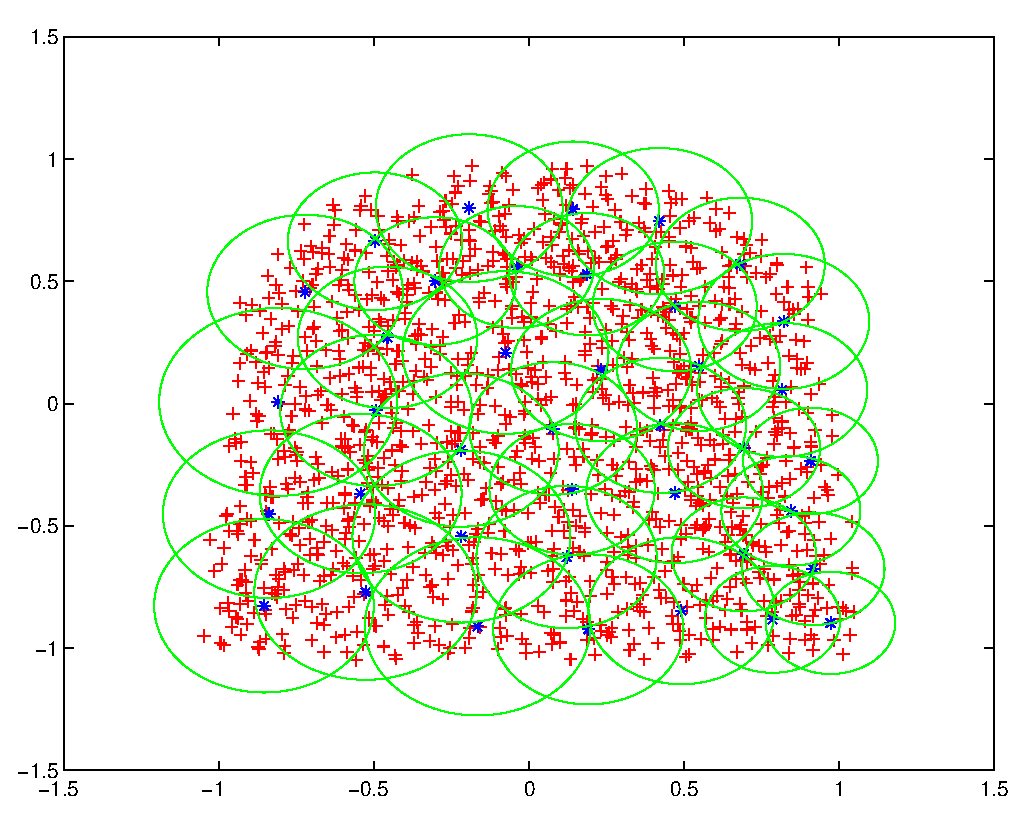
\includegraphics[width=\textwidth]{imagenes/complex-centroids}
            \caption{Vista de los radios y centroides obtenidos}
            \label{fig:complex-centroids}
    \end{subfigure}%
     %add desired spacing between images, e. g. ~, \quad, \qquad etc.
      %(or a blank line to force the subfigure onto a new line)
    \begin{subfigure}[b]{0.5\textwidth}
            \centering
            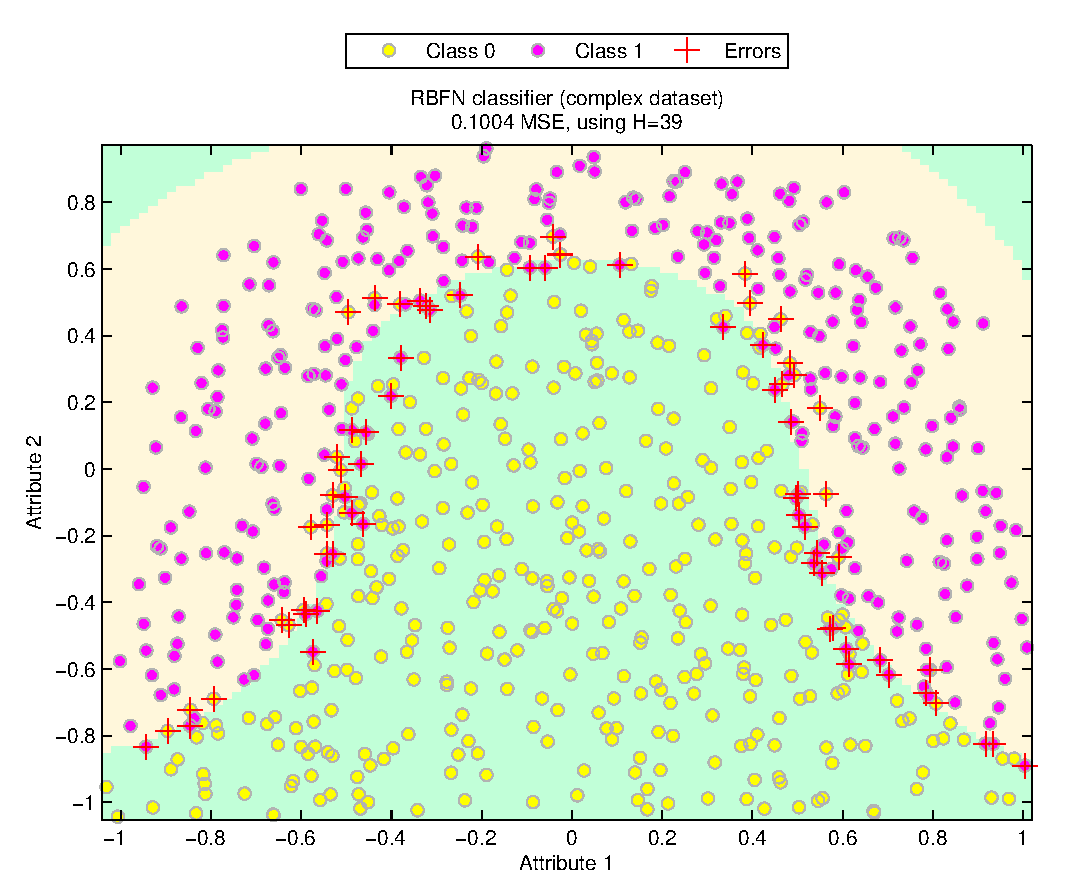
\includegraphics[width=\textwidth]{imagenes/complex}
            \caption{Espacio particionado de la mejor RBFN}
            \label{fig:complex-partition}
    \end{subfigure}
    \caption{Resultados obtenidos para el dataset \emph{complex}}\label{fig:espacio-particionado-complex}
\end{figure*}

% \begin{figure}[tb]
% 	\centering
% 	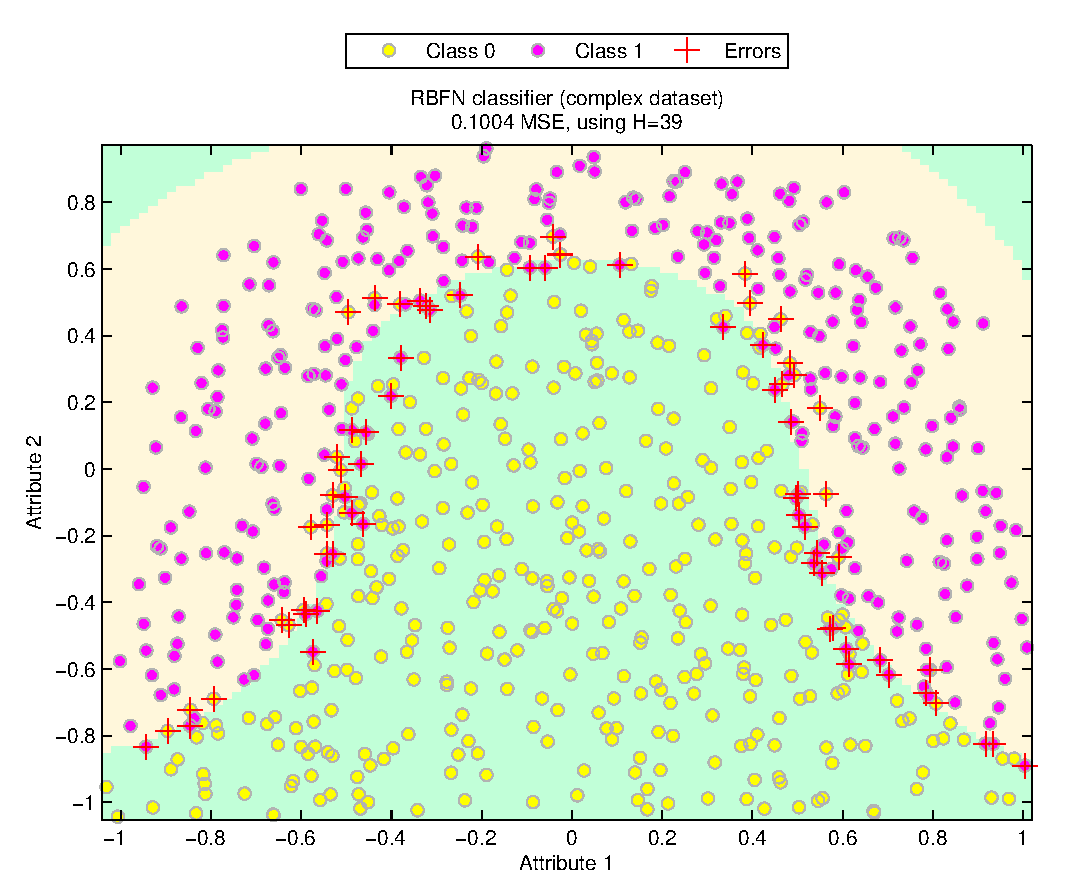
\includegraphics[width=\columnwidth]{imagenes/complex}
% 	\caption{Espacio particionado de la mejor RBFN para el dataset \emph{complex}}
% 	\label{fig:espacio-particionado-complex}
% \end{figure}


\begin{figure*}
\centering
    \begin{subfigure}[b]{0.5\textwidth}            
            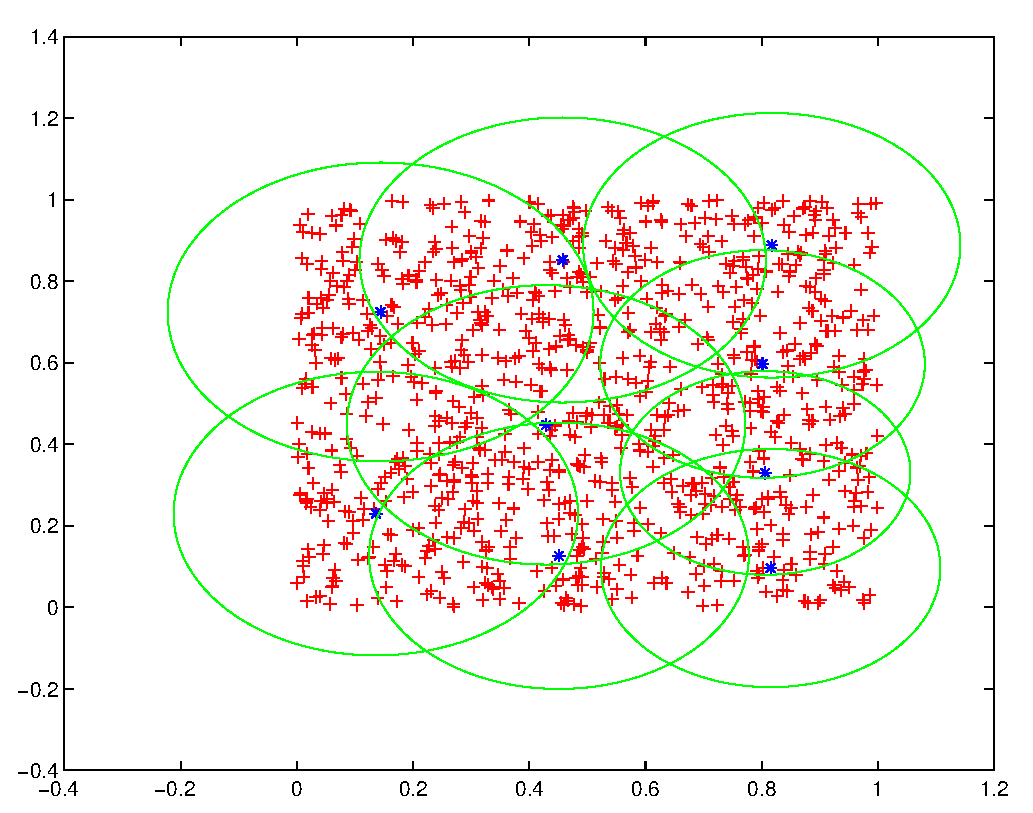
\includegraphics[width=\textwidth]{imagenes/linear-centroids}
            \caption{Vista de los radios y centroides obtenidos}
            \label{fig:linear-centroids}
    \end{subfigure}%
     %add desired spacing between images, e. g. ~, \quad, \qquad etc.
      %(or a blank line to force the subfigure onto a new line)
    \begin{subfigure}[b]{0.5\textwidth}
            \centering
            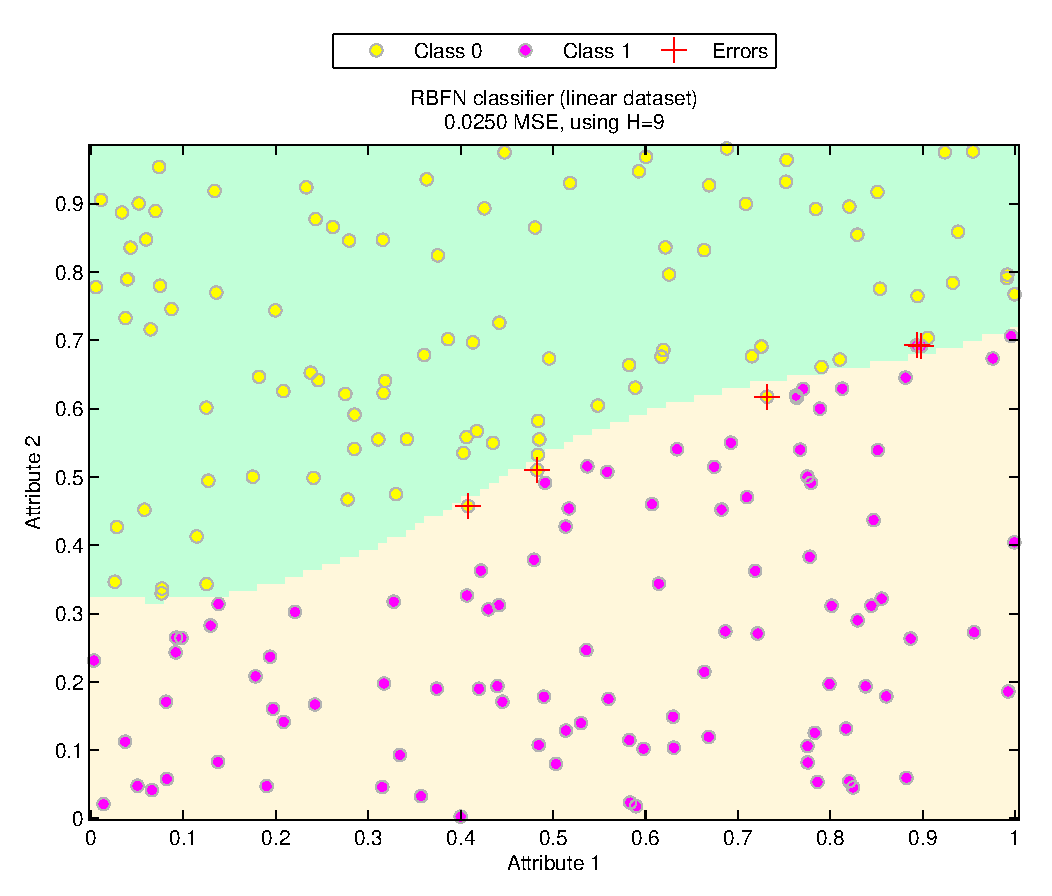
\includegraphics[width=\textwidth]{imagenes/linear}
            \caption{Espacio particionado de la mejor RBFN}
            \label{fig:linear-partition}
    \end{subfigure}
    \caption{Resultados obtenidos para el dataset \emph{linear}}\label{fig:espacio-particionado-linear}
\end{figure*}
% \begin{figure}[tb]
% 	\centering
% 	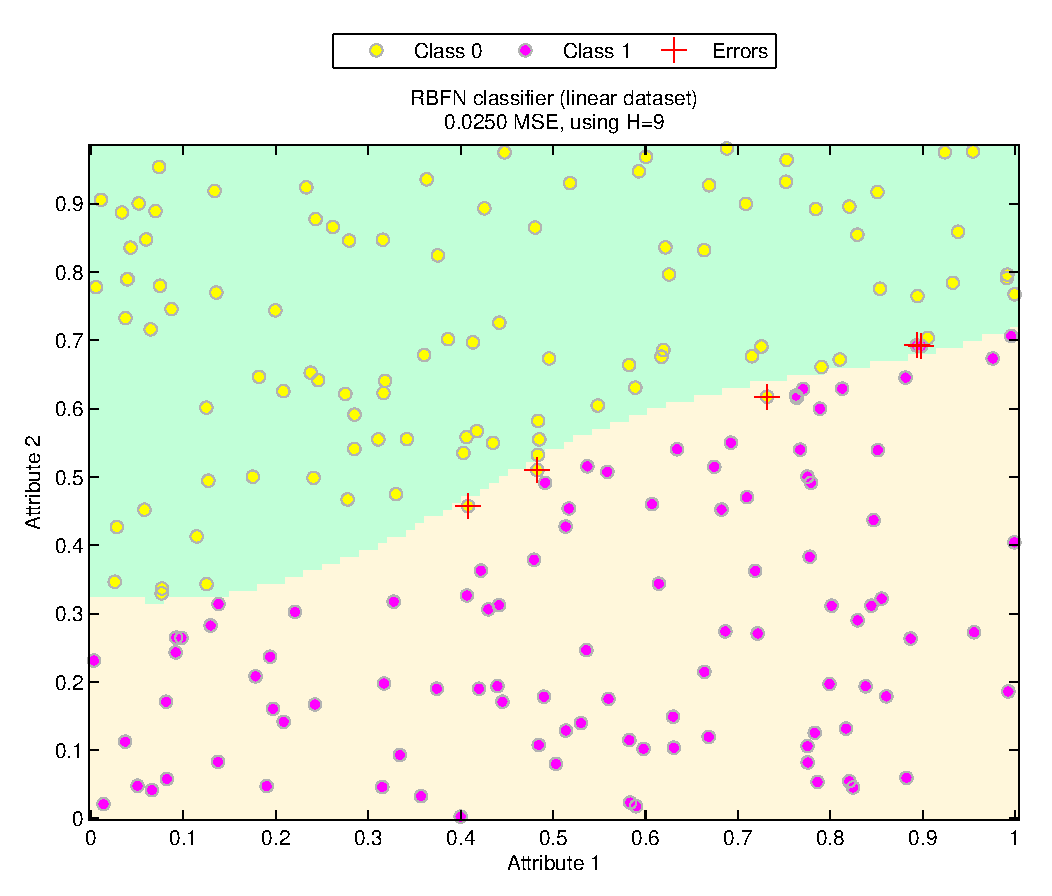
\includegraphics[width=\columnwidth]{imagenes/linear}
% 	\caption{Espacio particionado de la mejor RBFN para el dataset \emph{linear}}
% 	\label{fig:espacio-particionado-linear}
% \end{figure}


\begin{figure*}
\centering
    \begin{subfigure}[b]{0.5\textwidth}            
            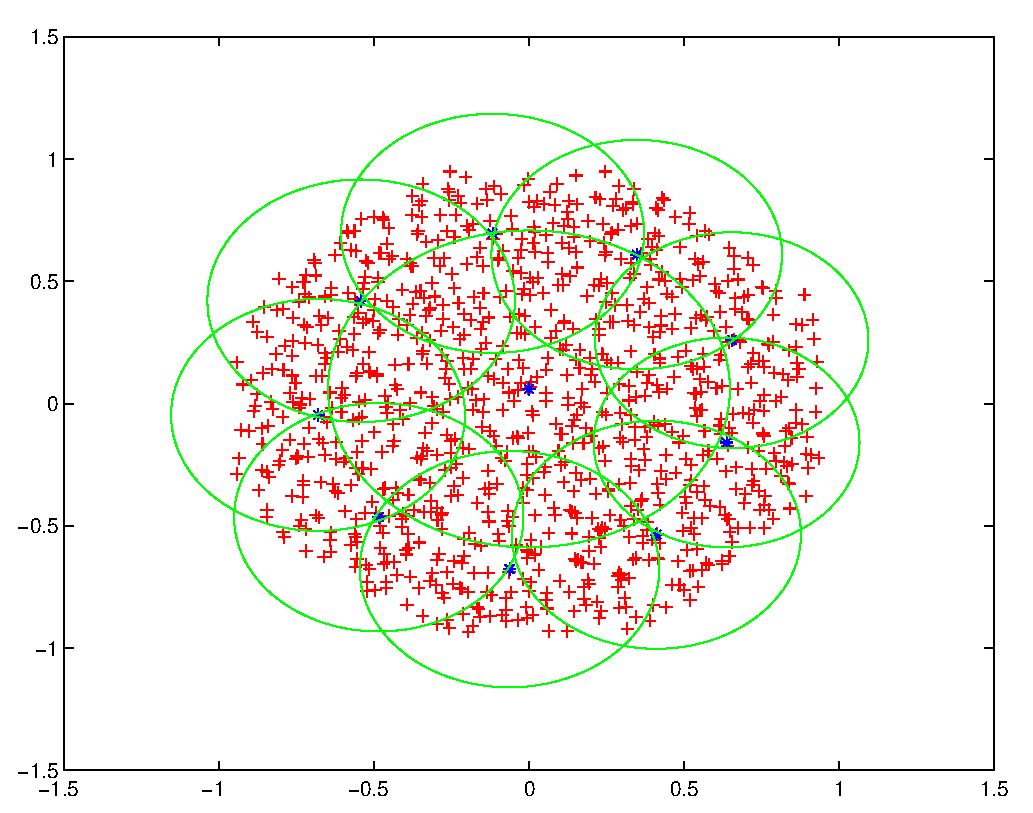
\includegraphics[width=\textwidth]{imagenes/ring-centroids}
            \caption{Vista de los radios y centroides obtenidos}
            \label{fig:ring-centroids}
    \end{subfigure}%
     %add desired spacing between images, e. g. ~, \quad, \qquad etc.
      %(or a blank line to force the subfigure onto a new line)
    \begin{subfigure}[b]{0.5\textwidth}
            \centering
            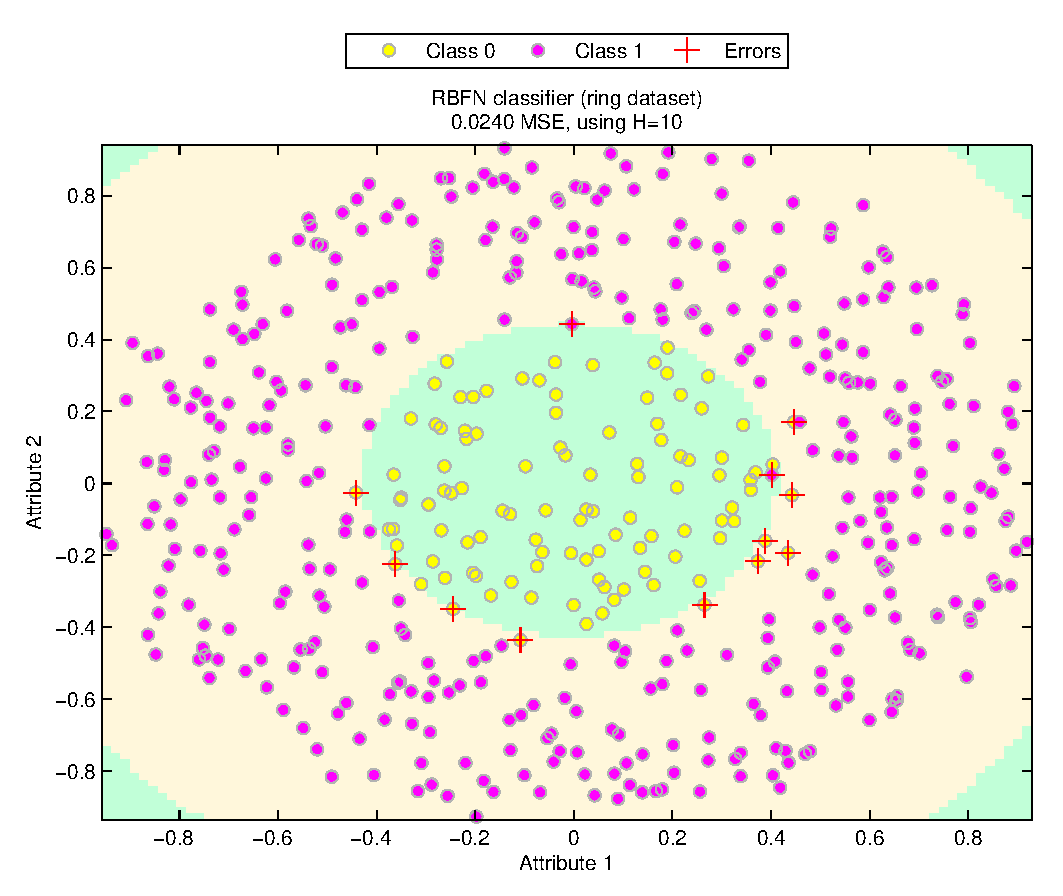
\includegraphics[width=\textwidth]{imagenes/ring}
            \caption{Espacio particionado de la mejor RBFN}
            \label{fig:ring-partition}
    \end{subfigure}
    \caption{Resultados obtenidos para el dataset \emph{ring}}\label{fig:espacio-particionado-ring}
\end{figure*}

% \begin{figure}[tb]
% 	\centering
% 	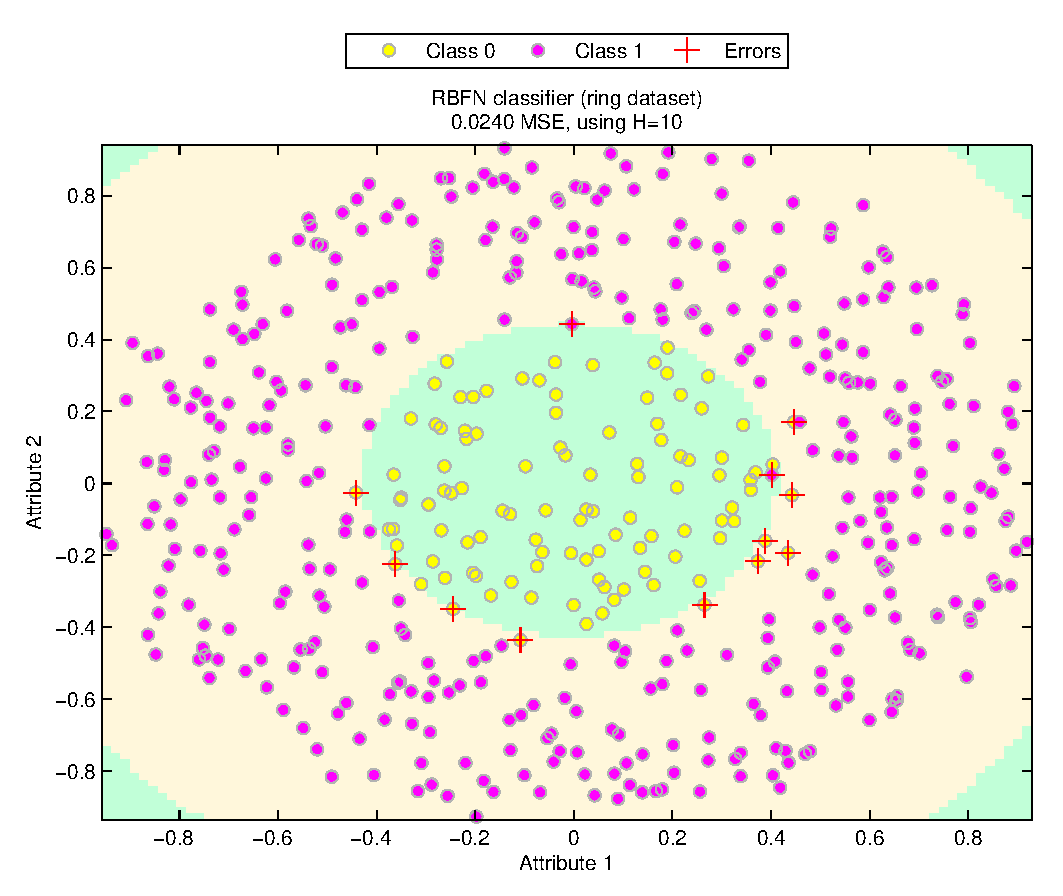
\includegraphics[width=\columnwidth]{imagenes/ring}
% 	\caption{Espacio particionado de la mejor RBFN para el dataset \emph{ring}}
% 	\label{fig:espacio-particionado-ring}
% \end{figure}

\begin{figure*}
\center
    \begin{subfigure}[b]{0.5\textwidth}            
            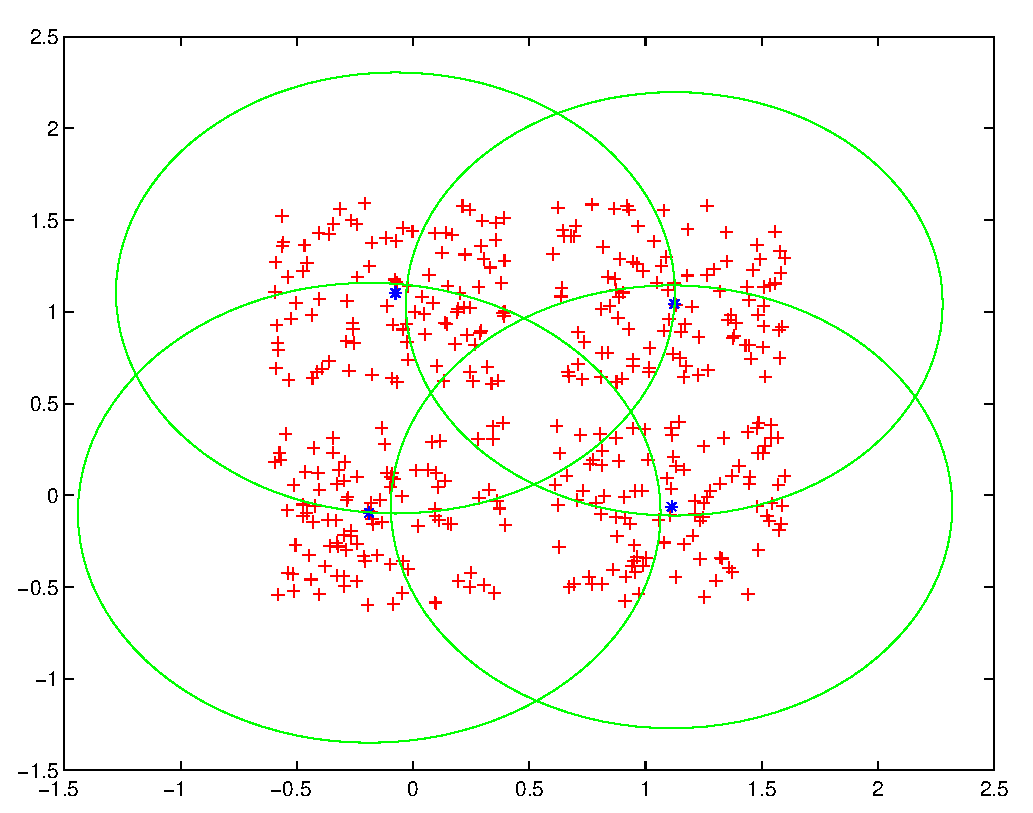
\includegraphics[width=\textwidth]{imagenes/xor-centroids}
            \caption{Vista de los radios y centroides obtenidos}
            \label{fig:xor-centroids}
    \end{subfigure}%
     %add desired spacing between images, e. g. ~, \quad, \qquad etc.
      %(or a blank line to force the subfigure onto a new line)
    \begin{subfigure}[b]{0.5\textwidth}
            \center
            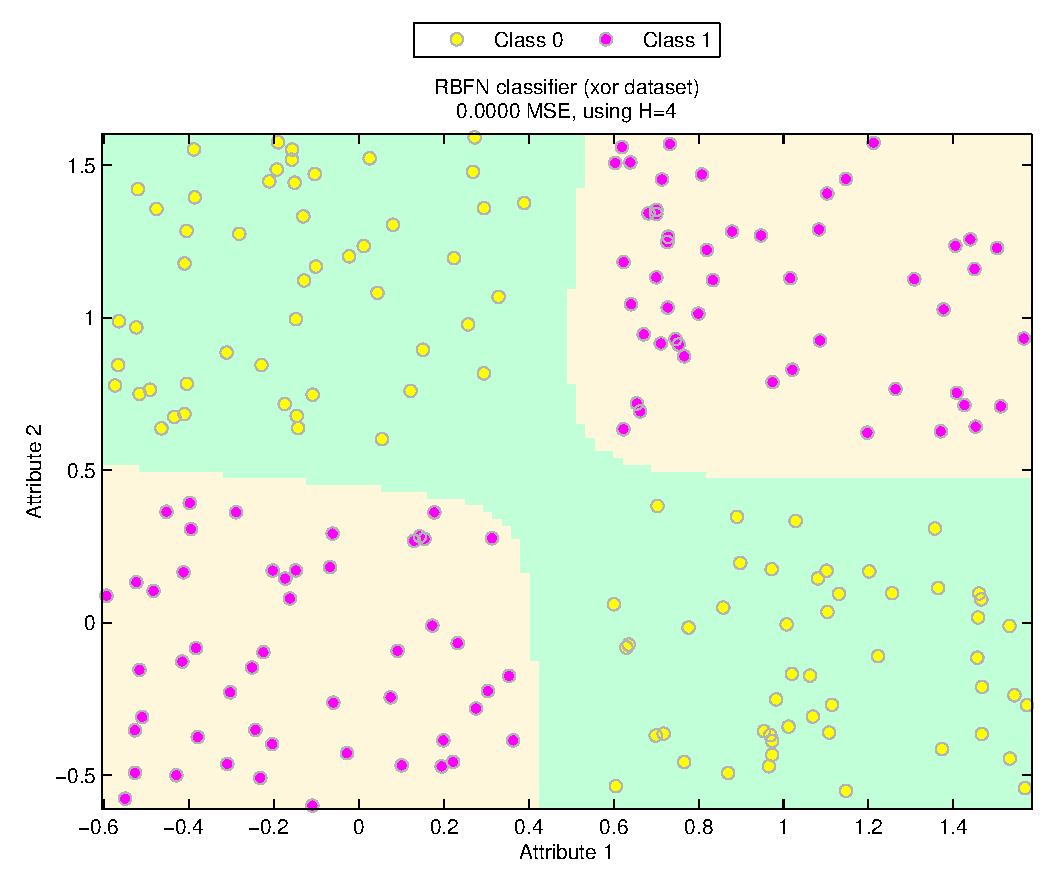
\includegraphics[width=\textwidth]{imagenes/xor}
            \caption{Espacio particionado de la mejor RBFN}
            \label{fig:xor-partition}
    \end{subfigure}
    \caption{Resultados obtenidos para el dataset \emph{xor}}\label{fig:espacio-particionado-xor}
\end{figure*}

% \begin{figure}[tb]
% 	\centering
% 	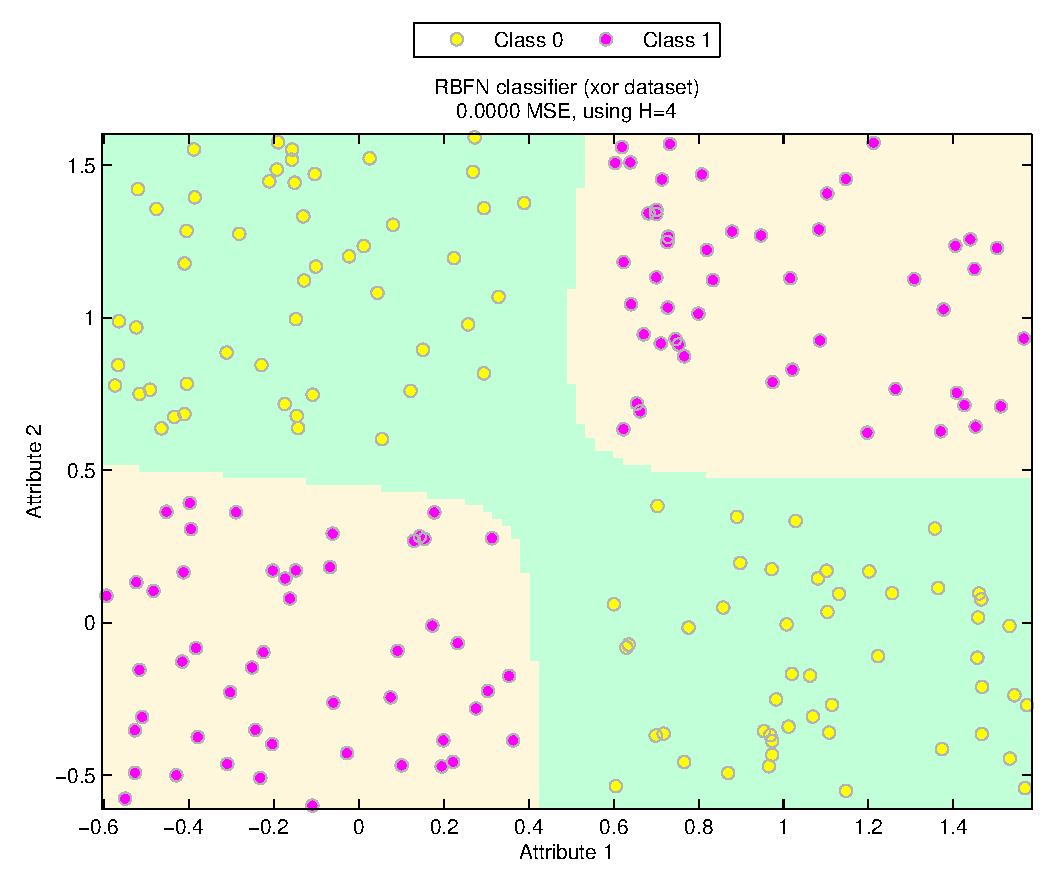
\includegraphics[width=\columnwidth]{imagenes/xor}
% 	\caption{Espacio particionado de la mejor RBFN para el dataset \emph{xor}}
% 	\label{fig:espacio-particionado-xor}
% \end{figure}


\section{Discusión de resultados}
\label{sec:discusion}
Las RBFN implementadas obtienen valores de error muy bajos para los datasets \emph{linear}, \emph{ring} y \emph{xor}.
Para el caso del dataset \emph{complex}, los resultados de error aumentan de forma considerable, tal como en el caso de las RNA MLP implementadas en la asignación anterior.

Un aspecto importante a destacar es la rapidez con la que la combinación de métodos entrega los resultados.
Fueron implementadas 31 ejecuciones para cada una de las configuraciones de parámetros.
Si bien es cierto que son menos que en la implementación de las RNA MLP de la asignación anterior, es evidente que la rapidez de las RBFN les posicionan como un mejor candidato (de acuerdo a los resultados de los datasets utilizados en esta práctica).

Adicionalmente, en el aspecto técnico este tipo de redes resultan más fáciles de implementar, considerando las facilidades provistas por \emph{Matlab}.



\section{Conclusiones}
\label{sec:conclusiones}
Las RBFN se presentan como una alternativa al perceptrón multicapa para labores de aproximación de funciones y clasificación de patrones.
Este tipo de redes definen una estructura fija de capas de entrada, oculta y de salida, siendo activadas las neuronas por una función no lineal, como por ejemplo la función Gaussiana.

Debido a su entrenamiento híbrido, algunas de las variantes de entrenamiento de las RBFN no requieren una iteración excesiva ni la retropropagación del error, por lo que su ejecución puede resultar más rápida.

Este documento ha descrito la implementación y resultados de la ejecución de RBFN con variaciones en la cantidad de neuronas y cálculos de radios, utilizando un entrenamiento híbrido con \emph{k-means} en la etapa no supervisada y el método de la matriz pseudoinversa en la etapa supervisada sobre cuatro datasets.
Los resultados indican que este tipo de redes pueden desempeñarse de forma más rápida y obtener mejores resultados (para los datasets considerados) en la clasificación que las redes de tipo MLP.

\nocite{*}
\bibliographystyle{IEEEtran}
\bibliography{referencias}

\end{document}

